\documentclass[final,t,overlay]{beamer}
\mode<presentation>
{
  \usetheme{UCL}
}
\usepackage[size=a0,scale=1,debug]{beamerposter}

% additional packages
\usepackage[english]{babel}
\usepackage[utf8]{inputenc}
\usepackage{pstool}
\usepackage{calc}
\usepackage{import}
\usepackage{color}
\usepackage{multicol}
\usepackage{graphicx}
\usepackage{tikz}
\usepackage{amsmath}
\usepackage{amsthm,amsthm}
\usepackage{amssymb}
\usetikzlibrary{arrows,shapes}
\tikzstyle{square}=[draw, minimum size=2.5em]
\tikzstyle{round}=[draw,circle, minimum size=2.5em]

 \def\mm#1{\ensuremath{\boldsymbol{#1}}} % version: amsmath
 
\DeclareMathOperator{\diag}{diag}
\DeclareMathOperator{\var}{var}
\DeclareMathOperator{\med}{Median}
\DeclareMathOperator{\chol}{cholesky}
\DeclareMathOperator{\tr}{tr}
\DeclareMathOperator*{\minimise}{minimise}
\DeclareMathOperator*{\argmax}{arg\,max}
\DeclareMathOperator*{\argmin}{arg\,min}

\global\long\def\Mz{M_{\mathbf{z},y}}
\global\long\def\muz{\mu_{\mathbf{z}}}
\global\long\def\aj{\alpha^{(j)}}
\global\long\def\ajt{\left(\alpha^{(j)}\right)^{\top}}

%empf is red now
%\renewcommand{\emph}[1]{{\color{red}{#1}}}

\title{A Kernel Test of Goodness of Fit}
\author[SHORTAUTHOR]
{Kacper Chwialkowski$^*$ Heiko Strathmann$^*$ Arthur Gretton}
\institute[SHORTINSTITUTE]{Gatsby Unit, University College London.}

\date[SHORTDATE]{DATE}

\global\long\def\ev{\mathbb{E}}

\newtheorem{thm}{Theorem}
\definecolor{mg}{rgb}{0,0.44,0}
\usepackage{graphicx}


\begin{document}
\begin{frame}
\begin{columns}
\begin{column}{.33\linewidth}
%\vspace{-0.75cm}
\begin{block}{Motivation: One sample testing for non i.i.d.\ data}
\begin{minipage}{.57\linewidth}

\begin{align*}
 \theta_{1}&\sim{\cal N}(0,10);\theta_{2}\sim{\cal N}(0,1) \\
 X_{i} &\sim\frac{1}{2}{\cal N}(\theta_{1},4)+\frac{1}{2}{\cal N}(\theta_{1}+\theta_{2},4)
\end{align*}
 \vspace{1cm} 

And so we turn the Bayesian Crank  to  obtain samples form the posteriori distribution. It obviously matters which matter which method we use, since quality of sample depends on it. However, once we are one  done one question remains...  
\end{minipage}
\begin{minipage}{.37\linewidth}
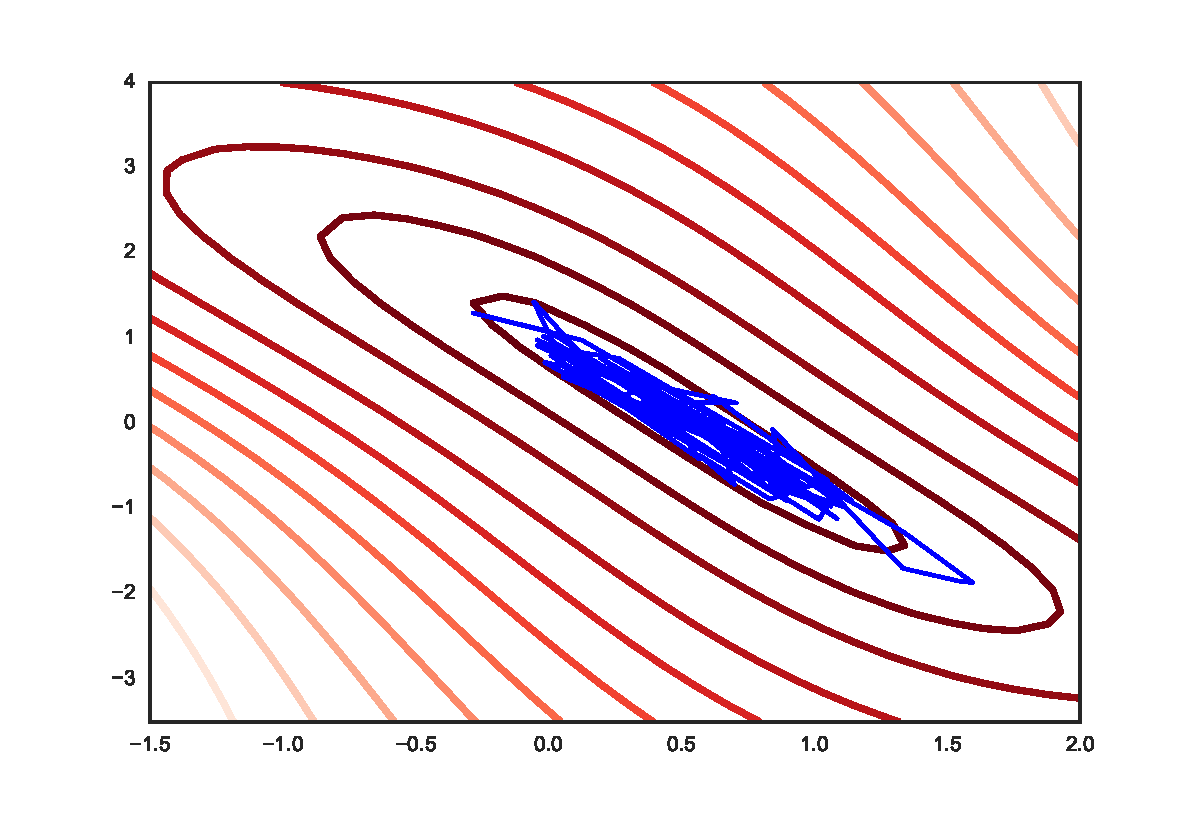
\includegraphics[scale=0.8]{../../presentation/img/sgld_trace_and_density.pdf}
\end{minipage}
\vspace{1cm}
\begin{center}
\Large
\emph{How to check if we sampled form the stationary distribution?}
\end{center}
\end{block}
\vspace{-0.75cm}
\begin{block}{So far: Maximum Mean Discrepancy}
\begin{center}We turn the Kernel Crank, we find a function in RKHS to reveal difference in distributions\end{center}
\begin{minipage}{.60\linewidth}


\vspace{1cm}
\large
\begin{align*}
MMD({\color{red} p},{ \color{blue} q},F) = \sup_{   \| {\color{mg}f} \|_F<1} [\ev_{{ \color{blue} q}}{\color{mg}f}- \ev_{{\color{red} p}}{\color{mg} f}]   
\end{align*}
\normalsize
\vspace{1cm}
 \begin{itemize}
  \item $F$ is an Reproducing Kernel Hilbert Space.
  \item ${\color{mg} f^*}$ is the function that attains the supremum.
  \item We want to get rid of  $\ev_{ {\color{red} p} }f$ . Hoe?
 \end{itemize}

\end{minipage}
\begin{minipage}{.35\linewidth}
\begin{center}
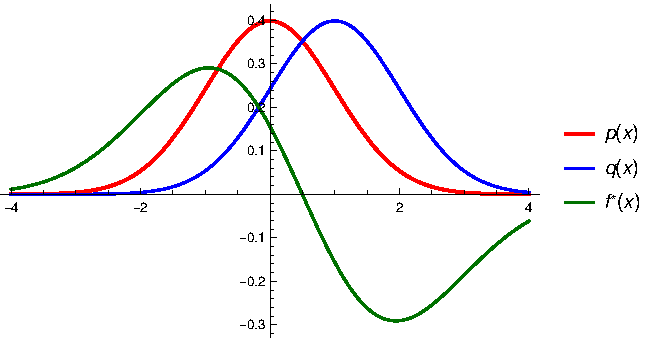
\includegraphics[width=12cm,height=6cm]{../../presentation/img/mmd.pdf}
\end{center}
\end{minipage}
\vspace{1cm}
\begin{center}
\emph{Can we do this without sampling from $p$?}
\end{center}
\end{block}
\vspace{-0.75cm}
\begin{block}{Stein's trick in RKHS}

Consider the  class \large
$$G = \{ f  +  \log' { \color{blue} q} \cdot  f | f \in F \}$$
\normalsize
justified by integration by parts
\begin{align*}
 0= &  f(x) {\color{red} p}(x)  \big|_{x=-\infty}^{x=\infty} =  \int_{-\infty}^{\infty} (f(x) {\color{red} p}(x) )'  dx  =   \int   f(x)' { \color{blue} q}(x)   + f(x){\color{red} p}'(x)  = \ev_{\color{red} p} f(X)  +  \log' {\color{red} p}(X) f(X) \\
   = & \ev_{\color{red} p} g(X), \\
    & \quad \quad \quad  \quad  \text{ where } g \in G
\end{align*}

\end{block}
\vspace{-0.75cm}

\begin{block}{Stein discrepancy}
\large
\begin{align*}
MMD({\color{red} p},{ \color{blue} q},G) = \sup_{   \| {\color{mg} g} \|_G<1} \ev_{{ \color{blue} q}}{\color{mg}g} - \ev_{{\color{red} p}} {\color{mg}g}  = \sup_{ \| {\color{mg} g} \|_G<1} \ev_{{ \color{blue} q}} {\color{mg}g} 
\end{align*}
\vspace{2cm}
\centering
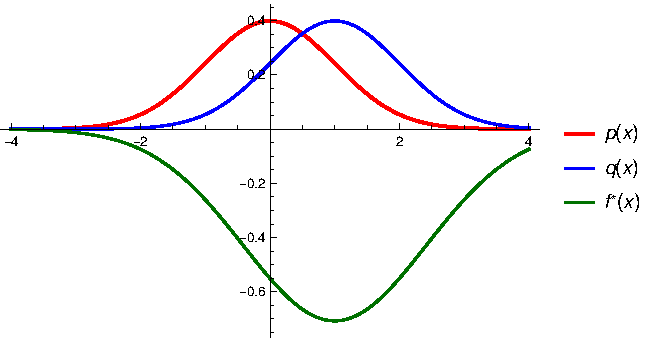
\includegraphics[scale=1.2]{../../presentation/img/s1.pdf}
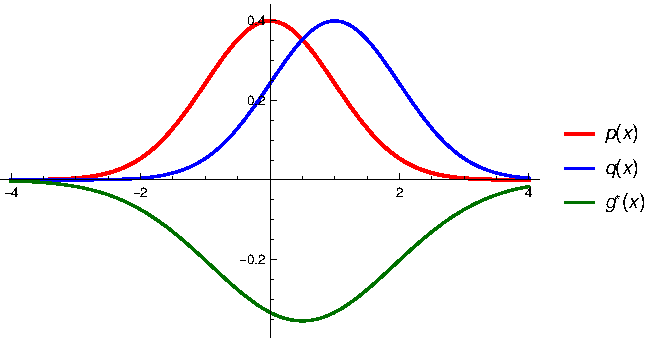
\includegraphics[scale=1.2]{../../presentation/img/s05.pdf}\\
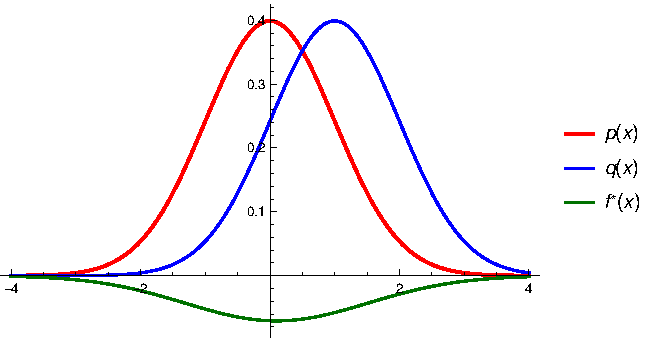
\includegraphics[scale=1.2]{../../presentation/img/s01.pdf}
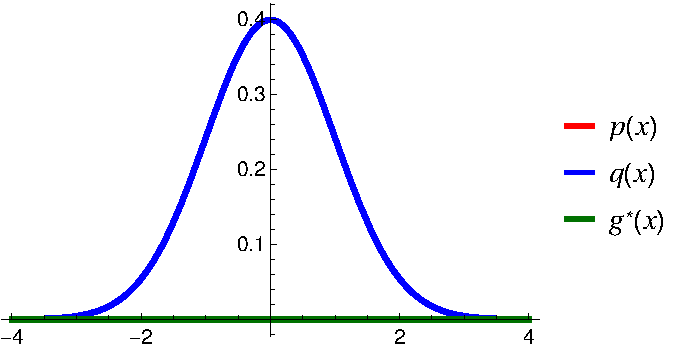
\includegraphics[scale=1.2]{../../presentation/img/s0.pdf}
%%\includegraphics[width=10cm, height=7cm]{../../presentation/img/old/figures/kmc/gaussian_trajectories_momentum_hmc}
%\includegraphics[scale=1.2]{../../presentation/img/old/figures/kmc/gaussian_trajectories_acceptance_hmc}\\

%\includegraphics[scale=.5]{../../presentation/img/old/figures/kmc/kmc_banana_bbox}
%%\includegraphics[width=10cm, height=7cm]{../../presentation/img/old/figures/kmc/gaussian_trajectories_momentum_kmc}
%\includegraphics[scale=1.2]{../../presentation/img/old/figures/kmc/gaussian_trajectories_acceptance_kmc}
\vspace{1cm}
\begin{center}
\emph{Bam!}
\end{center}
\end{block}
\end{column}

%%%-----------------column 2
\hspace{-1.45cm}
\begin{column}{.33\linewidth}

%\vspace{-0.75cm}
\begin{block}{Closed form expression}
 Let $F$ be the RKHS associated with the kernel $k$. Consider a friendly looking function
\begin{align*}
h_{{\color{red} p}}(x,y) & := \partial_{x} \log {\color{red} p}(x) \partial_{x} \log {\color{red} p}(y) k(x,y)\\
 & \quad+\partial_{y} \log {\color{red} p}(y) \partial_{x}  k(x,y)\\
 & \quad+\partial_{x} \log {\color{red} p}(x) \partial_{y}k(x,y)\\
 & \quad+\partial_{x} \partial_{y} k(x,y).
\end{align*}
 \center{\emph{Only depends on kernel and $\partial_{x} \log {\color{red} p}(x)$}}
 
\end{block}

\vspace{-0.75cm}
\begin{block}{Theorem}
\large
Let ${ \color{blue} q},{\color{red} p}$ be probability measures and $Z\sim { \color{blue} q}$. 
If $\ev_{{ \color{blue} q}} h_{{\color{red} p}}(Z,Z)<\infty$, then $MMD({\color{red} p},{ \color{blue} q},G) = \ev_{{ \color{blue} q}} h_{{\color{red} p}}(Z,Z')$.
\end{block}
\vspace{-0.75cm}
\begin{block}{Theorem}
\large
If the kernel $k$ is cc-universal, $\ev_{{ \color{blue} q}} h_{{ \color{blue} q}}(Z,Z)<\infty$ and $\ev_{{ \color{blue} q}} (\log' \frac{{\color{red} p}(Z)}{{ \color{blue} q}(Z)})^{2}<\infty$
then $MMD({\color{red} p},{ \color{blue} q},G) =0$ if and only if ${\color{red} p}={ \color{blue} q}$.

\end{block}
\vspace{-0.75cm}
\begin{block}{Estimation: V-statistics}
An estimator of $\ev h_{\color{red} p}(X,X')$ is
\begin{align*}
 V_n(h_{\color{red} p}) = \frac {1} {n^2} \sum_{i,j=1}^n h_{\color{red} p}(X_i,X_j).
\end{align*}
Our test statistic is $ n V_n(h_{\color{red} p})$.

If $X_i \sim {\color{red} p}$ then $ n V_n(h_{\color{red} p})$  converges weakly. 

Otherwise it does not,  it explodes, $P(n V_n(h_{\color{red} p}) <C) \to 0$.
\end{block}
\vspace{-0.75cm}
\begin{block}{Non i.i.d.\ extension: the wild bootstrap}
To estimate quantiles of $ V_n(h_{\color{red} p})$  
\[
 V_n(h_{\color{red} p}) = \frac {1} {n^2} \sum_{i,j=1}^n h_{\color{red} p}(X_i,X_j).
\]
under the null, we use wild bootstrap
\[
 B_n(h_{\color{red} p}) = \frac {1} {n^2} \sum_{i,j=1}^n W_i W_j h_{\color{red} p}(X_i,X_j).
\]
  where $W_i$ is a specific series of zero valued random variables.


 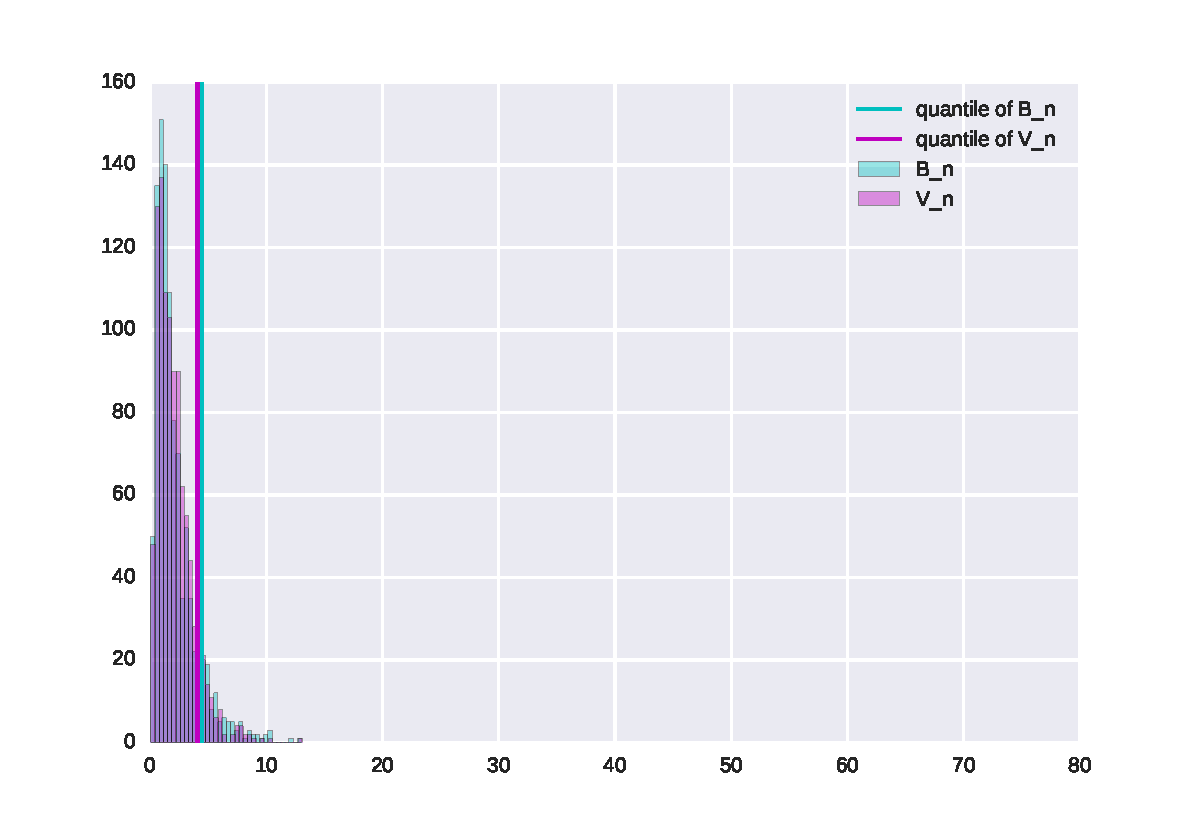
\includegraphics[width=0.3\textwidth]{../../presentation/img/bootstrapWorks1.pdf}
 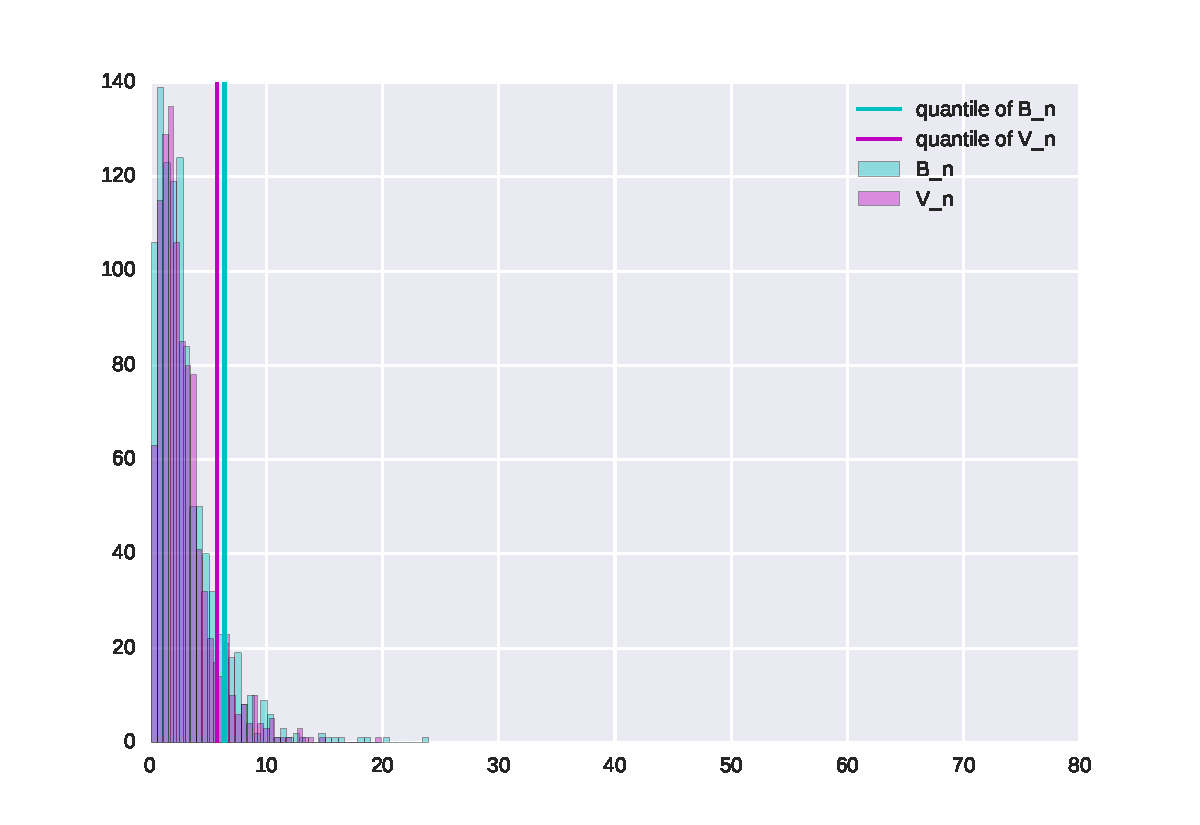
\includegraphics[width=0.3\textwidth]{../../presentation/img/bootstrapWorks4.pdf}
 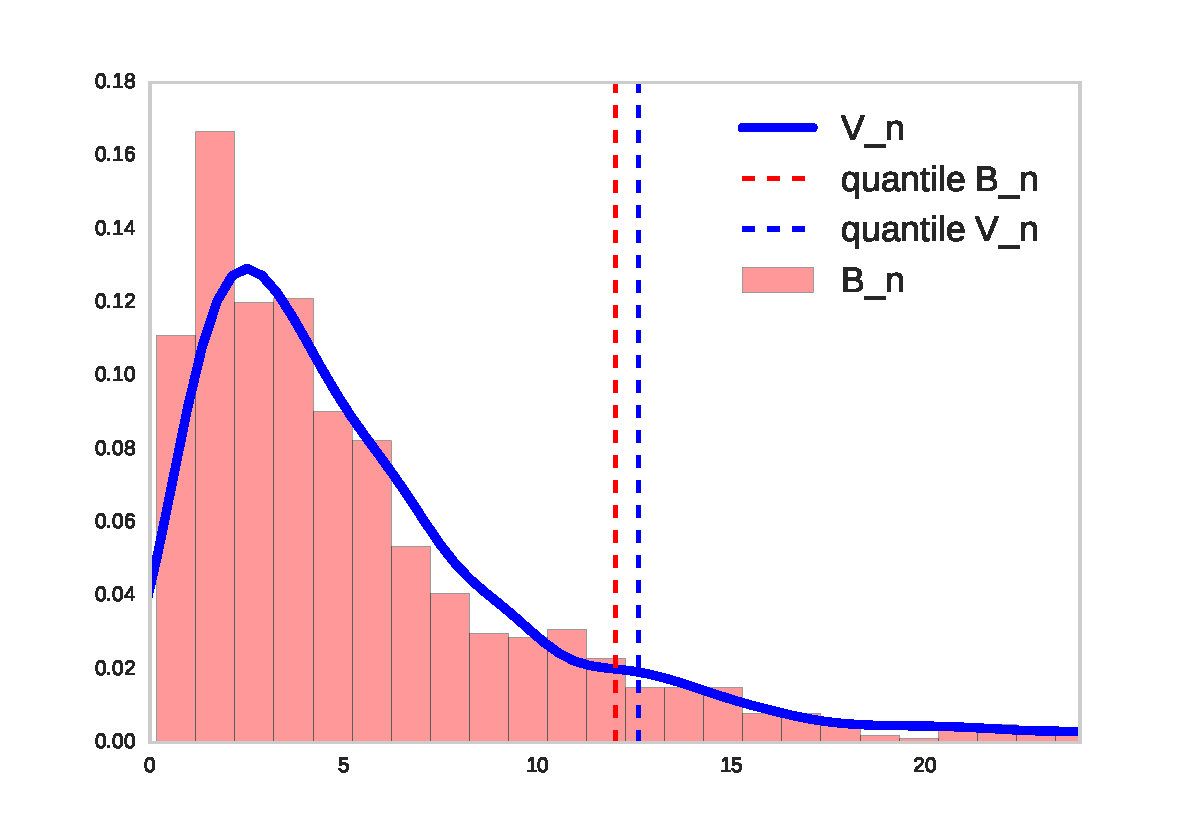
\includegraphics[width=0.3\textwidth]{../../presentation/img/bootstrapWorks7.pdf}
\end{block}
\end{column}


% column 3
\hspace{-1.45cm}
\begin{column}{.32\linewidth}
%\vspace{-0.75cm}
\begin{block}{Experiment: Student's T vs.\ Normal}
\begin{minipage}{.60\linewidth}
\begin{itemize}
\item TODO Describe
\end{itemize}
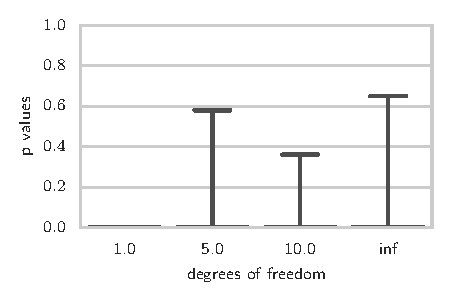
\includegraphics[width=.7\textwidth]{../../presentation/img/sgld_student_bad}
\end{minipage}
\begin{minipage}{.35\linewidth}
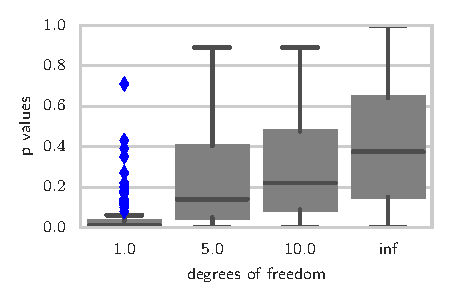
\includegraphics[width=1\textwidth]{../../presentation/img/sgld_student}\\
 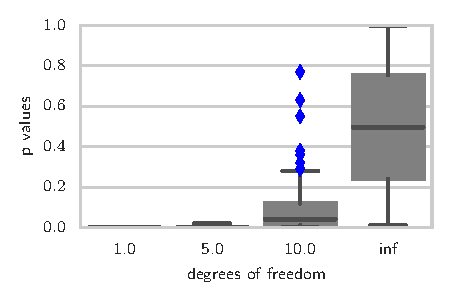
\includegraphics[width=1\textwidth]{../../presentation/img/sgld_student_opt} 
\end{minipage}
\end{block}
\vspace{-0.75cm}
\begin{block}{Experiment: Bias quantification in Approximate MCMC}
\begin{minipage}{.60\linewidth}
\begin{align*}
\theta_{1}\sim{\cal N}(0,10);\theta_{2}\sim{\cal N}(0,1)\\
X_{i}\sim\frac{1}{2}{\cal N}(\theta_{1},4)+\frac{1}{2}{\cal N}(\theta_{1}+\theta_{2},4) & .
\end{align*}
\begin{center}
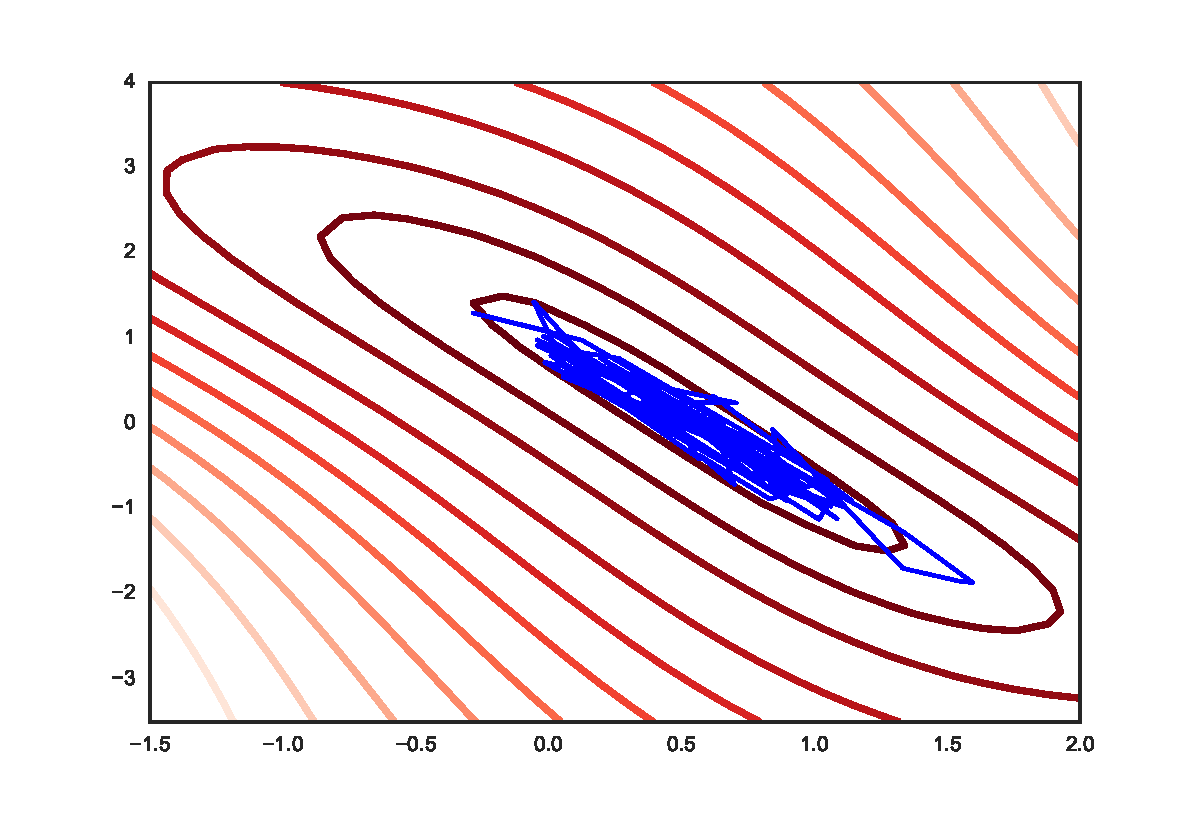
\includegraphics[width=0.5\textwidth]{../../presentation/img/sgld_trace_and_density.pdf}
\end{center}
\end{minipage}
\begin{minipage}{.35\linewidth}
           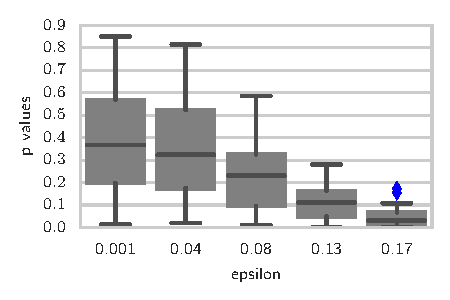
\includegraphics[width=.6\textwidth]{../../presentation/img/Heiko1}\\
            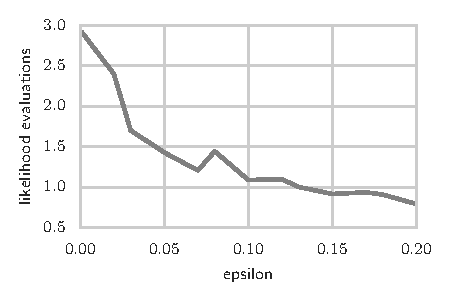
\includegraphics[width=.6\textwidth]{../../presentation/img/Heiko2}
\end{minipage}
\end{block}
\vspace{-0.75cm}
\begin{block}{Experiment: Statistical model criticism}
\begin{center}
\item We test the hypothesis that a Gaussian process generated \textbf{training data} using for fitting -- without simulating from the generative model, but only using {\color{red} test data}.
\end{center}
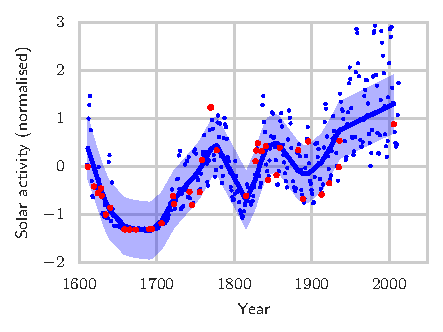
\includegraphics[width=0.48\textwidth]{../../presentation/img/gp_regression_data_fit.pdf} 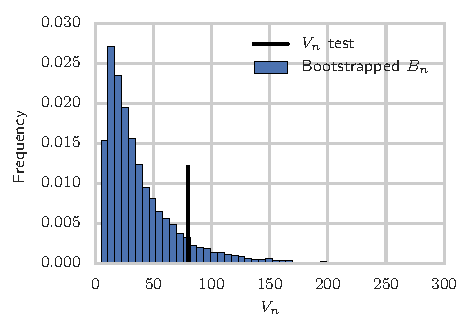
\includegraphics[width=0.48\textwidth]{../../presentation/img/gp_regression_bootstrap_hist} 
\begin{minipage}{.35\linewidth}

\end{minipage}
\end{block}
\vspace{-0.75cm}
\begin{block}{References}
\begin{minipage}{.9\linewidth}
{\footnotesize
\begin{multicols}{2}
\setbeamertemplate{bibliography item}[text] 
\bibliographystyle{plain} 
\scriptsize
\bibliography{../../biblio.bib} \ 
\end{multicols}
} 
\end{minipage}
\end{block}

\end{column}
\end{columns}

\end{frame}
\end{document}
